\chapter[Resultados Individuais]{Resultados Individuais (Por Empresa)}

\section{Considerações Iniciais}

Em nossa pesquisa, para as 8 empresas que participaram, 3 delas atingiram o número mínimo de respostas que permitem uma análise individual da empresa (10 avaliações de desenvolvedores). Nós iremos mostrar nesse capítulo o resultado que obtivemos analisando essas 3 empresas. Para proteger as informações dessas empresas, elas não serão identificadas. Nos referenciaremos à elas então como “Empresa A”, “Empresa B” e “Empresa C”.

\section{Análise das Empresas}

Para cada uma das 3 empresas, faremos a análise utilizando os dois conjuntos de classes, apontando as diferenças nos resultados. Mostraremos então a distribuição dos desenvolvedores ao longo dos dois conjuntos de classes, a seleção de características executadas no conjunto de dados resultantes da pesquisa respondida pelos supervisores das respectivas empresas e o resultado da aplicação dos algoritmos de classificação (dados de diferentes times, porém pertencentes à mesma empresa foram mesclados para obtermos uma visão geral da empresa).

Assim como fizemos com o conjunto de dados que representava todas as empresas, aplicamos aqui os algoritmos de classificação J48 e NaïveBayes nos dados fornecidos pelas respectivas empresas, utilizando tanto o conjunto original de classes quanto o novo conjunto de classes. 

Como explicado na seção \ref{secao3.4}, para associar a seleção de características com os algoritmos de classificação da maneira correta, utilizaremos o Algoritmo AttributeSelectedClassifier, usando o algoritmo GainRatioAttributeEval para selecionar os atributos mais relevantes. E da mesma maneira que foi realizado a seleção de características ao analisarmos o conjunto de dados de todas as empresas (apresentado na seção \ref{secao4.4}), a quantidade de características ideal que maximiza a acurácia dos classificadores é escolhida através de um teste exaustivo, começando com apenas duas características e aumentando uma a uma até chegar nas dezesseis características apresentadas na \autoref{tabela2} (já começamos com um número maior que 1 pois o objetivo não é encontrar correlação de alguma característica em específico com a classe, e sim encontrar um padrão na combinação de características que se correlacione com a importância dada pelo supervisor).

\subsection{Análise da Empresa A}

\subsubsection{Pesquisa}

A empresa A obteve avaliações de 2 supervisores. Como eram times com propósitos bem diferentes, consideramos apenas as avaliações de um dos times para representar a Empresa A, visto que o segundo não obteve avaliações suficientes para ser analisado individualmente. Logo, o time avaliado obteve 19 avaliações de desenvolvedores. A \autopageref{fig_7} e a \autoref{fig_8} mostram a distribuição dos desenvolvedores pelo conjunto de classes original e pelo novo conjunto de classes, respectivamente.


\begin{figure}[p]
	\centering
	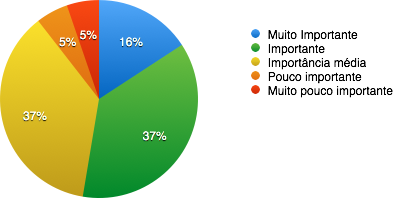
\includegraphics[width=\textwidth]{figs/empresa_a/imagem-classe-original.png}
	\caption{\label{fig_7}Distribuição dos desenvolvedores pelo conjunto original de classes (Empresa A)}
\end{figure}

\begin{figure}[p]
	\centering
	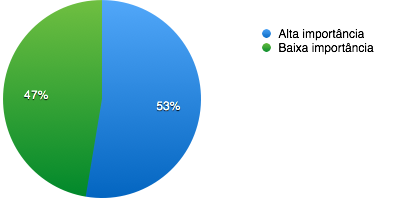
\includegraphics[width=\textwidth]{figs/empresa_a/imagem-classe-alternativa.png}
	\caption{\label{fig_8}Distribuição dos desenvolvedores pelo novo conjunto de classes (Empresa A)}
\end{figure}

\subsubsection{Seleção de Características}
O resultado da aplicação do algoritmo de seleção de características para o conjunto original de classes e para o novo conjunto de classes é apresentado na \autoref{tabela8} e na \autoref{tabela9} respectivamente.

%inserir Tabela 8
\begin{table}[h]
	\caption{Ordenação dos atributos da Empresa A (conjunto original de 5 classes)}
	\label{tabela8}
	\def\arraystretch{2}
	\begin{tabular}{|p{8.5cm}|>{\centering\arraybackslash}p{3cm}|>{\centering\arraybackslash}p{3cm}|}
		\hline
		\textbf{Atributos}                                                      & \textbf{Posição média} & \textbf{Mérito médio} \\ \hline
		Capacidade de resolução de problemas complexos                          & 1.5 +- 0.81            & 0.582 +- 0.038        \\ \hline
		Foco nos resultados                                                     & 2.6 +- 1.02            & 0.519 +- 0.047        \\ \hline
		Criatividade                                                            & 3 +- 1                 & 0.504 +- 0.035        \\ \hline
		Pró-atividade                                                           & 5.1 +- 2.12            & 0.456 +- 0.048        \\ \hline
		Foco no cliente                                                         & 6.4 +- 1.96            & 0.437 +- 0.04         \\ \hline
		Diversidade de habilidades                                              & 6.5 +- 1.91            & 0.435 +- 0.025        \\ \hline
		Experiência relevante                                                   & 6.9 +- 2.39            & 0.427 +- 0.035        \\ \hline
		Conhecimento especializado                                              & 8.9 +- 3.05            & 0.396 +- 0.053        \\ \hline
		PRINCIPAL comportamento do desenvolvedor                                & 9.4 +- 2.91            & 0.384 +- 0.058        \\ \hline
		Qual a sua avaliação sobre a produtividade do desenvolvedor em questão? & 9.8 +- 2.44            & 0.383 +- 0.041        \\ \hline
		Comunicação com os colegas                                              & 10.5 +- 2.16           & 0.371 +- 0.051        \\ \hline
		Empreendedorismo                                                        & 11.7 +- 1.79           & 0.351 +- 0.047        \\ \hline
		Disposição para ajudar colegas quando solicitado                        & 12.1 +- 2.62           & 0.348 +- 0.05         \\ \hline
		Organização e planejamento                                              & 12.6 +- 2.24           & 0.336 +- 0.042        \\ \hline
		Tempo de trabalho (meses)                                               & 14.5 +- 4.5            & 0.064 +- 0.192        \\ \hline
		Liderança                                                               & 14.5 +- 0.81           & 0.285 +- 0.063        \\ \hline
	\end{tabular}
\end{table}
\clearpage

%inserir Tabela 9
\begin{table}[h]
	\caption{Ordenação dos atributos da Empresa A (novo conjunto de classes)}
	\label{tabela9}
	\def\arraystretch{2}
	\begin{tabular}{|p{8.5cm}|>{\centering\arraybackslash}p{3cm}|>{\centering\arraybackslash}p{3cm}|}
		\hline
		\textbf{Atributos}                                                      & \textbf{Posição média} & \textbf{Mérito médio} \\ \hline
		Pró-atividade                                                           & 1.2 +- 0.4             & 0.323 +- 0.021        \\ \hline
		Capacidade de resolução de problemas complexos                          & 2.4 +- 0.8             & 0.298 +- 0.032        \\ \hline
		Comunicação com os colegas                                              & 4 +- 1.48              & 0.254 +- 0.024        \\ \hline
		Foco nos resultados                                                     & 5 +- 1.48              & 0.23 +- 0.029         \\ \hline
		Criatividade                                                            & 6.7 +- 1.68            & 0.206 +- 0.025        \\ \hline
		Qual a sua avaliação sobre a produtividade do desenvolvedor em questão? & 7.5 +- 2.01            & 0.187 +- 0.026        \\ \hline
		Organização e planejamento                                              & 7.8 +- 3.22            & 0.191 +- 0.035        \\ \hline
		Conhecimento especializado                                              & 8.2 +- 3.28            & 0.189 +- 0.056        \\ \hline
		Experiência relevante                                                   & 9.2 +- 3.12            & 0.173 +- 0.04         \\ \hline
		Empreendedorismo                                                        & 10.2 +- 3.22           & 0.171 +- 0.037        \\ \hline
		PRINCIPAL comportamento do desenvolvedor                                & 10.4 +- 3.8            & 0.172 +- 0.052        \\ \hline
		Disposição para ajudar colegas quando solicitado                        & 11.1 +- 4.35           & 0.156 +- 0.049        \\ \hline
		Foco no cliente                                                         & 11.2 +- 1.72           & 0.158 +- 0.02         \\ \hline
		Liderança                                                               & 13 +- 2.53             & 0.137 +- 0.039        \\ \hline
		Diversidade de habilidades                                              & 13.4 +- 3.1            & 0.136 +- 0.046        \\ \hline
		Tempo de trabalho (meses)                                               & 14.7 +- 1.68           & 0.123 +- 0.022        \\ \hline
	\end{tabular}
\end{table}
\clearpage
\subsubsection{Classificação}

A \autoref{tabela10} e a \autoref{tabela11} apresentam os melhores resultados obtidos através da aplicação dos algoritmos J48 e NaïveBayes nos dados da Empresa A, respectivamente. Os algoritmos foram aplicados em ambos conjunto original de 5 classes e no novo conjunto de classes. 

A \autoref{fig_9} e a \autoref{fig_10} mostram a aplicação exaustiva do algoritmo que associa a seleção de características com os algoritmos de classificação, para o J48 e para o NaïveBayes respectivamente.

Observando o teste exaustivo do J48, pudemos notar que ele obteve uma melhor performance utilizando um pequeno número de características ao realizar a classificação. No caso do conjunto original de 5 classes, os melhores resultados foram obtidos selecionando de 2 a 4 características, e ao ser aplicado utilizando o novo conjunto de classes, a melhor acurácia foi obtida selecionando apenas 2 características. É importante ressaltar também o aumento de aproximadamente 20\% na acurácia do classificador utilizando a segunda classe de dados.

Diferentemente do J48, o NaïveBayes obteve uma melhor performance ao selecionar um maior número de características, de 13 a 15 no conjunto original de classes e acima de 7 no novo conjunto de classes. O NaïveBayes também teve uma melhoria de performance considerável ao utilizar o novo conjunto de dados (11\%).

%inserir Tabela 10
\begin{table}[h]
	\caption{Aplicação do J48 para os diferentes conjuntos de classe da Empresa A}
	\label{tabela10}
	\def\arraystretch{1.5}
	\begin{tabular}{|p{7.25cm}|>{\centering\arraybackslash}p{7.25cm}|}
		\hline
		\textbf{Classe}                         & \textbf{Porcentagem de acertos} \\ \hline
		\textbf{Conjunto original de 5 classes} & 59\%                         \\ \hline
		\textbf{Novo conjunto de classes}       & 79.50\%                         \\ \hline
	\end{tabular}
\end{table}

%inserir Tabela 11
\begin{table}[h]
	\caption{Aplicação do NaïveBayes para os diferentes conjuntos de classe da Empresa A}
	\label{tabela11}
	\def\arraystretch{1.5}
	\begin{tabular}{|p{7.25cm}|>{\centering\arraybackslash}p{7.25cm}|}
		\hline
		\textbf{Classe}                         & \textbf{Porcentagem de acertos} \\ \hline
		\textbf{Conjunto original de 5 classes} & 68.50\%                         \\ \hline
		\textbf{Novo conjunto de classes}       & 79.50\%                         \\ \hline
	\end{tabular}
\end{table}

\begin{figure}[p]
	\centering
	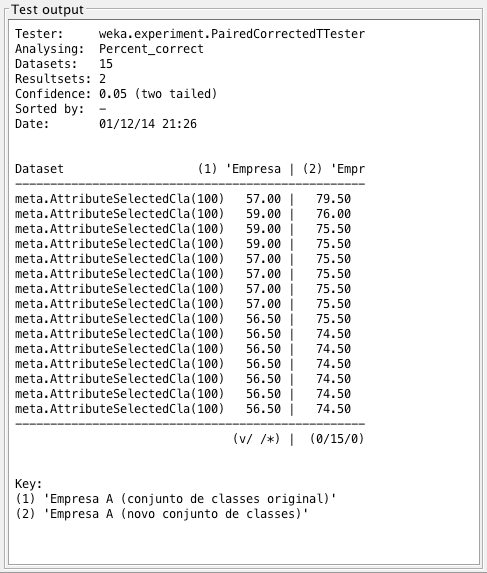
\includegraphics[width=\textwidth]{figs/empresa_a/exaustive-j48.png}
	\caption{\label{fig_9}Aplicação exaustiva do J48 para a Empresa A}
\end{figure}
\clearpage

\begin{figure}[p]
	\centering
	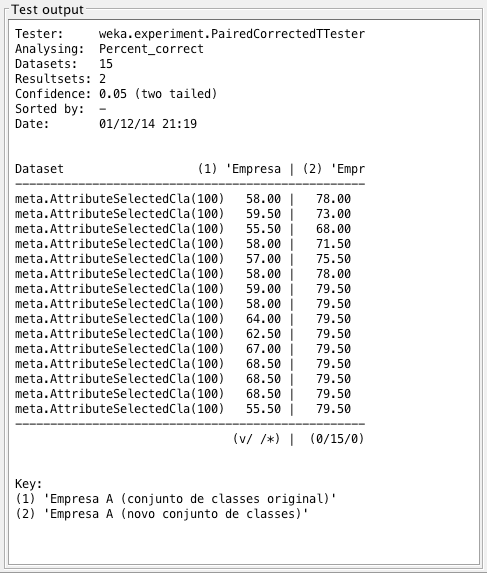
\includegraphics[width=\textwidth]{figs/empresa_a/exaustive-naivebayes.png}
	\caption{\label{fig_10}Aplicação exaustiva do NaïveBayes para a Empresa A}
\end{figure}
\clearpage

\subsection{Análise da Empresa B}

\subsubsection{Pesquisa}

A Empresa B obteve 10 avaliações de desenvolvedores feitas por um único supervisor. A \autoref{fig_11} e a \autoref{fig_12} mostram a distribuição dos desenvolvedores pelo conjunto de classes original e pelo novo conjunto de classes, respectivamente.

\begin{figure}[p]
	\centering
	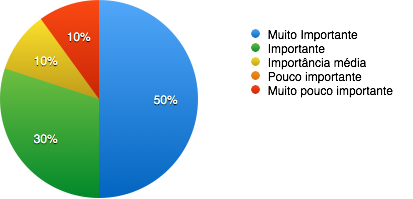
\includegraphics[width=\textwidth]{figs/empresa_b/imagem-classe-original.png}
	\caption{\label{fig_11}Distribuição dos desenvolvedores pelo conjunto original de classes (Empresa B)}
\end{figure}

\begin{figure}[p]
	\centering
	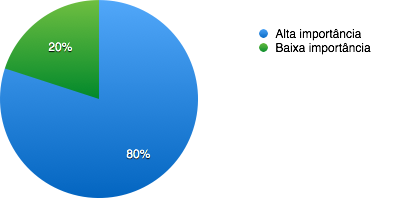
\includegraphics[width=\textwidth]{figs/empresa_b/imagem-classe-alternativa.png}
	\caption{\label{fig_12}Distribuição dos desenvolvedores pelo novo conjunto de classes (Empresa B)}
\end{figure}

\subsubsection{Seleção de Características}
O resultado da aplicação do algoritmo de seleção de características para o conjunto original de classes e para o novo conjunto de classes é apresentado na \autoref{tabela12} e na \autoref{tabela13} respectivamente.

%inserir Tabela 12
\begin{table}[h]
	\caption{Ordenação dos atributos da Empresa B (conjunto original de 5 classes)}
	\label{tabela12}
	\def\arraystretch{2}
	\begin{tabular}{|p{8.5cm}|>{\centering\arraybackslash}p{3cm}|>{\centering\arraybackslash}p{3cm}|}
		\hline
		\textbf{Atributos}                                                      & \textbf{Posição média} & \textbf{Mérito médio} \\ \hline
		Capacidade de resolução de problemas complexos                          & 1.3 +- 0.46            & 0.772 +- 0.078        \\ \hline
		Liderança                                                               & 2.4 +- 1.02            & 0.652 +- 0.118        \\ \hline
		Tempo de trabalho (meses)                                               & 4.6 +- 1.43            & 0.562 +- 0.063        \\ \hline
		Foco nos resultados                                                     & 5 +- 3.63              & 0.611 +- 0.179        \\ \hline
		Experiência relevante                                                   & 5.3 +- 3.29            & 0.611 +- 0.179        \\ \hline
		Organização e planejamento                                              & 6.4 +- 1.8             & 0.506 +- 0.073        \\ \hline
		Conhecimento especializado                                              & 6.7 +- 2.1             & 0.515 +- 0.094        \\ \hline
		Diversidade de habilidades                                              & 8 +- 1.48              & 0.456 +- 0.06         \\ \hline
		Criatividade                                                            & 9.7 +- 2.79            & 0.413 +- 0.119        \\ \hline
		Qual a sua avaliação sobre a produtividade do desenvolvedor em questão? & 11.1 +- 2.43           & 0.361 +- 0.076        \\ \hline
		Pró-atividade                                                           & 11.2 +- 1.54           & 0.35 +- 0.04          \\ \hline
		Foco no cliente                                                         & 11.2 +- 4.04           & 0.373 +- 0.133        \\ \hline
		Empreendedorismo                                                        & 11.4 +- 1.74           & 0.36 +- 0.079         \\ \hline
		Disposição para ajudar colegas quando solicitado                        & 12.4 +- 1.85           & 0.339 +- 0.08         \\ \hline
		Comunicação com os colegas                                              & 13.6 +- 2.15           & 0.318 +- 0.087        \\ \hline
		PRINCIPAL comportamento do desenvolvedor                                & 15.7 +- 0.64           & 0.235 +- 0.048        \\ \hline
	\end{tabular}
\end{table}
\clearpage

%inserir Tabela 13
\begin{table}[h]
	\caption{Ordenação dos atributos da Empresa B (novo conjunto de classes)}
	\label{tabela13}
	\def\arraystretch{2}
	\begin{tabular}{|p{8.5cm}|>{\centering\arraybackslash}p{3cm}|>{\centering\arraybackslash}p{3cm}|}
		\hline
		\textbf{Atributos}                                                      & \textbf{Posição média} & \textbf{Mérito médio} \\ \hline
		Foco nos resultados                                                     & 2.9 +- 4.41            & 0.327 +- 0.131        \\ \hline
		Comunicação com os colegas                                              & 3.3 +- 1.42            & 0.244 +- 0.067        \\ \hline
		Experiência relevante                                                   & 3.4 +- 4.25            & 0.327 +- 0.131        \\ \hline
		Criatividade                                                            & 4.1 +- 2.07            & 0.26 +- 0.069         \\ \hline
		Capacidade de resolução de problemas complexos                          & 5.6 +- 1.56            & 0.151 +- 0.052        \\ \hline
		Pró-atividade                                                           & 8.1 +- 3.14            & 0.112 +- 0.028        \\ \hline
		PRINCIPAL comportamento do desenvolvedor                                & 8.1 +- 3.18            & 0.112 +- 0.028        \\ \hline
		Tempo de trabalho (meses)                                               & 8.6 +- 2.29            & 0.109 +- 0.033        \\ \hline
		Diversidade de habilidades                                              & 8.6 +- 3.5             & 0.119 +- 0.06         \\ \hline
		Qual a sua avaliação sobre a produtividade do desenvolvedor em questão? & 9.4 +- 1.74            & 0.093 +- 0.022        \\ \hline
		Empreendedorismo                                                        & 9.6 +- 1.85            & 0.093 +- 0.022        \\ \hline
		Disposição para ajudar colegas quando solicitado                        & 11.3 +- 1.42           & 0.063 +- 0.02         \\ \hline
		Conhecimento especializado                                              & 12.7 +- 1.42           & 0.043 +- 0.026        \\ \hline
		Organização e planejamento                                              & 12.9 +- 2.84           & 0.031 +- 0.043        \\ \hline
		Foco no cliente                                                         & 13.3 +- 3.23           & 0.031 +- 0.043        \\ \hline
		Liderança                                                               & 14.1 +- 3.67           & 0.023 +- 0.04         \\ \hline
	\end{tabular}
\end{table}
\clearpage

\subsubsection{Classificação}

A \autoref{tabela14} e a \autoref{tabela15} apresentam os melhores resultados obtidos através da aplicação dos algoritmos J48 e NaïveBayes nos dados da empresa B, respectivamente. Os algoritmos foram aplicados em ambos conjunto original de 5 classes e no novo conjunto de classes.

A \autoref{fig_13} e a \autoref{fig_14} mostram a aplicação exaustiva do algoritmo que associa a seleção de características com os algoritmos de classificação, para o J48 e para o NaïveBayes respectivamente.

Observando o teste exaustivo do J48, pudemos notar que, para o conjunto de classes original, o algoritmo obteve uma melhor performance utilizando um menor número de características (de 2 a 6). Já ao utilizar o novo conjunto de classes, o classificador obteve a mesma acurácia independentemente do número de características utilizado. Utilizando o segundo conjunto de classes, o J48 teve um aumento de 10\% em sua acurácia final.

No caso da Empresa B, o algoritmo NaïveBayes obteve uma performance extremamente semelhante ao J48, mantendo a performance praticamente constante de acordo com a variação das características selecionadas, obtendo uma melhoria de 10\% ao utilizar o novo conjunto de classes, e obtendo uma acurácia final de 80\%. 

%inserir Tabela 14
\begin{table}[h]
	\caption{Aplicação do J48 para os diferentes conjuntos de classe da Empresa B}
	\label{tabela14}
	\def\arraystretch{1.5}
	\begin{tabular}{|p{7.25cm}|>{\centering\arraybackslash}p{7.25cm}|}
		\hline
		\textbf{Classe}                         & \textbf{Porcentagem de acertos} \\ \hline
		\textbf{Conjunto original de 5 classes} & 70\%                         \\ \hline
		\textbf{Novo conjunto de classes}       & 80\%                         \\ \hline
	\end{tabular}
\end{table}

%inserir Tabela 15
\begin{table}[h]
	\caption{Aplicação do NaïveBayes para os diferentes conjuntos de classe da Empresa B}
	\label{tabela15}
	\def\arraystretch{1.5}
	\begin{tabular}{|p{7.25cm}|>{\centering\arraybackslash}p{7.25cm}|}
		\hline
		\textbf{Classe}                         & \textbf{Porcentagem de acertos} \\ \hline
		\textbf{Conjunto original de 5 classes} & 70\%                         \\ \hline
		\textbf{Novo conjunto de classes}       & 80\%                         \\ \hline
	\end{tabular}
\end{table}

\begin{figure}[p]
	\centering
	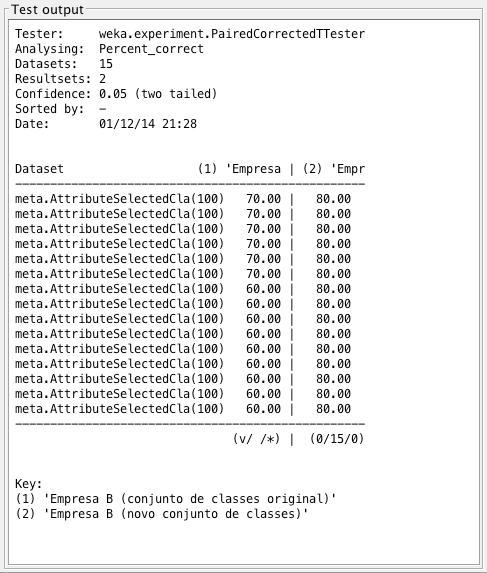
\includegraphics[width=\textwidth]{figs/empresa_b/exaustive-j48.png}
	\caption{\label{fig_13}Aplicação exaustiva do J48 para a Empresa B}
\end{figure}
\clearpage

\begin{figure}[p]
	\centering
	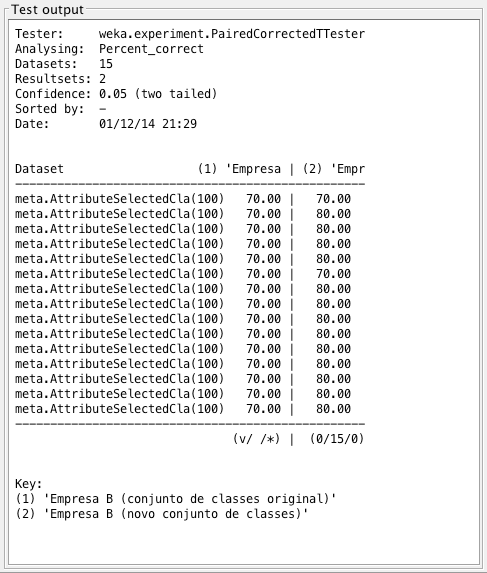
\includegraphics[width=\textwidth]{figs/empresa_b/exaustive-naivebayes.png}
	\caption{\label{fig_14}Aplicação exaustiva do NaïveBayes para a Empresa B}
\end{figure}
\clearpage


\subsection{Análise da Empresa C}

\subsubsection{Pesquisa}

A Empresa C obteve 18 avaliaçãos de desenvolvedores, dadas por 2 diferentes supervisores. Apesar de serem times diferentes, ambos fazem parte da mesma indústria de software, por isso resolvemos mesclar os dados e fazer uma avaliação conjunta. A Empresa C também obteve mais 2 avaliações dadas por um terceiro supervisor, mas os dados foram excluídos dessa análise pelo propósito desse time ser bastante diferente dos dois primeiros. A \autoref{fig_15} e a \autoref{fig_16} mostram a distribuição dos desenvolvedores pelo conjunto de classes original e pelo novo conjunto de classes, respectivamente. 

\begin{figure}[p]
	\centering
	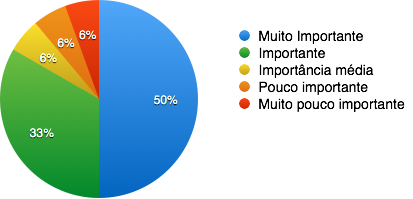
\includegraphics[width=\textwidth]{figs/empresa_c/imagem-classe-original.png}
	\caption{\label{fig_15}Distribuição dos desenvolvedores pelo conjunto original de classes (Empresa C)}
\end{figure}

\begin{figure}[p]
	\centering
	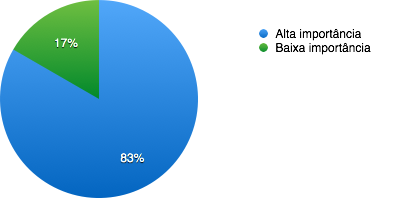
\includegraphics[width=\textwidth]{figs/empresa_c/imagem-classe-alternativa.png}
	\caption{\label{fig_16}Distribuição dos desenvolvedores pelo novo conjunto de classes (Empresa C)}
\end{figure}

\subsubsection{Seleção de Características}
O resultado da aplicação do algoritmo de seleção de características para o conjunto original de classes e para o novo conjunto de classes é apresentado na \autoref{tabela16} e na \autoref{tabela17} respectivamente.

%inserir Tabela 16
\begin{table}[h]
	\caption{Ordenação dos atributos da Empresa C (conjunto original de 5 classes)}
	\label{tabela16}
	\def\arraystretch{2}
	\begin{tabular}{|p{8.5cm}|>{\centering\arraybackslash}p{3cm}|>{\centering\arraybackslash}p{3cm}|}
		\hline
		\textbf{Atributos}                                                      & \textbf{Posição média} & \textbf{Mérito médio} \\ \hline
		Capacidade de resolução de problemas complexos                          & 1.1 +- 0.3             & 0.643 +- 0.044        \\ \hline
		Experiência relevante                                                   & 2.2 +- 0.4             & 0.581 +- 0.037        \\ \hline
		Conhecimento especializado                                              & 3.3 +- 0.9             & 0.518 +- 0.058        \\ \hline
		Qual a sua avaliação sobre a produtividade do desenvolvedor em questão? & 3.4 +- 0.66            & 0.504 +- 0.036        \\ \hline
		Diversidade de habilidades                                              & 5.2 +- 0.6             & 0.386 +- 0.046        \\ \hline
		PRINCIPAL comportamento do desenvolvedor                                & 6.4 +- 0.8             & 0.338 +- 0.048        \\ \hline
		Comunicação com os colegas                                              & 8.1 +- 1.45            & 0.301 +- 0.029        \\ \hline
		Foco nos resultados                                                     & 8.5 +- 2.77            & 0.3 +- 0.08           \\ \hline
		Empreendedorismo                                                        & 9.6 +- 2.06            & 0.275 +- 0.037        \\ \hline
		Pró-atividade                                                           & 10.7 +- 2              & 0.267 +- 0.058        \\ \hline
		Tempo de trabalho (meses)                                               & 11.2 +- 1.66           & 0.261 +- 0.035        \\ \hline
		Foco no cliente                                                         & 11.3 +- 1.68           & 0.255 +- 0.045        \\ \hline
		Criatividade                                                            & 11.9 +- 2.55           & 0.246 +- 0.056        \\ \hline
		Liderança                                                               & 13.6 +- 2.01           & 0.21 +- 0.055         \\ \hline
		Organização e planejamento                                              & 14.2 +- 1.54           & 0.196 +- 0.042        \\ \hline
		Disposição para ajudar colegas quando solicitado                        & 15.3 +- 0.78           & 0.186 +- 0.044        \\ \hline
	\end{tabular}
\end{table}
\clearpage

%inserir Tabela 17
\begin{table}[h]
	\caption{Ordenação dos atributos da Empresa C (novo conjunto de classes)}
	\label{tabela17}
	\def\arraystretch{2}
	\begin{tabular}{|p{8.5cm}|>{\centering\arraybackslash}p{3cm}|>{\centering\arraybackslash}p{3cm}|}
		\hline
		\textbf{Atributos}                                                      & \textbf{Posição média} & \textbf{Mérito médio} \\ \hline
		Conhecimento especializado                                              & 1 +- 0                 & 0.26 +- 0.028         \\ \hline
		Experiência relevante                                                   & 2.3 +- 0.46            & 0.24 +- 0.026         \\ \hline
		Qual a sua avaliação sobre a produtividade do desenvolvedor em questão? & 3.1 +- 0.83            & 0.227 +- 0.035        \\ \hline
		Capacidade de resolução de problemas complexos                          & 4 +- 0.45              & 0.216 +- 0.029        \\ \hline
		Diversidade de habilidades                                              & 5.6 +- 0.66            & 0.179 +- 0.027        \\ \hline
		Disposição para ajudar colegas quando solicitado                        & 6 +- 1.55              & 0.172 +- 0.034        \\ \hline
		Foco nos resultados                                                     & 7.1 +- 1.51            & 0.16 +- 0.03          \\ \hline
		Pró-atividade                                                           & 8.1 +- 1.97            & 0.147 +- 0.026        \\ \hline
		Tempo de trabalho (meses)                                               & 8.7 +- 1               & 0.133 +- 0.024        \\ \hline
		Organização e planejamento                                              & 10 +- 1                & 0.115 +- 0.025        \\ \hline
		Foco no cliente                                                         & 10.8 +- 1.4            & 0.091 +- 0.028        \\ \hline
		Criatividade                                                            & 12 +- 1.41             & 0.076 +- 0.015        \\ \hline
		Comunicação com os colegas                                              & 13.2 +- 0.75           & 0.064 +- 0.011        \\ \hline
		Liderança                                                               & 14.4 +- 1.62           & 0.048 +- 0.015        \\ \hline
		Empreendedorismo                                                        & 14.5 +- 1.02           & 0.048 +- 0.015        \\ \hline
		PRINCIPAL comportamento do desenvolvedor                                & 15.2 +- 1.08           & 0.041 +- 0.015        \\ \hline
	\end{tabular}
\end{table}
\clearpage

\subsubsection{Classificação}
A \autoref{tabela18} e a \autoref{tabela19} apresentam os melhores resultados obtidos através da aplicação dos algoritmos J48 e NaïveBayes nos dados da empresa C, respectivamente. Os algoritmos foram aplicados em ambos conjunto original de 5 classes e no novo conjunto de classes. 

A \autoref{fig_17} e a \autoref{fig_18} mostram a aplicação exaustiva do algoritmo que associa a seleção de características com os algoritmos de classificação, para o J48 e para o NaïveBayes respectivamente.

Observando o teste exaustivo do J48, pudemos notar que ele obteve uma melhor performance utilizando apenas 2 características ao realizar a classificação utilizando o primeiro conjunto de classes. Já ao utilizar o novo conjunto de classes, o classificador obteve a mesma acurácia independentemente do número de características utilizado. Utilizando o segundo conjunto de classes, o J48 teve um aumento de 8\% em sua acurácia final.

Diferentemente do J48, o NaïveBayes, ao utilizar o primeiro conjunto de classes obteve melhor performance selecionando um número mais intermediário de características (7). Já ao utilizar o novo conjunto de classes, o classificador atingiu sua acurácia máxima utilizando 2 ou 3 características, um número relativamente baixo. Nesse caso, o algoritmo obteve um ganho de performance de quase 15\% se comparado com quando utilizou o conjunto original de classes.


%inserir Tabela 18
\begin{table}[h]
	\caption{Aplicação do J48 para os diferentes conjuntos de classe da Empresa C}
	\label{tabela18}
	\def\arraystretch{1.5}
	\begin{tabular}{|p{7.25cm}|>{\centering\arraybackslash}p{7.25cm}|}
		\hline
		\textbf{Classe}                         & \textbf{Porcentagem de acertos} \\ \hline
		\textbf{Conjunto original de 5 classes} & 77\%                         \\ \hline
		\textbf{Novo conjunto de classes}       & 85\%                         \\ \hline
	\end{tabular}
\end{table}

%inserir Tabela 19
\begin{table}[h]
	\caption{Aplicação do NaïveBayes para os diferentes conjuntos de classe da Empresa C}
	\label{tabela19}
	\def\arraystretch{1.5}
	\begin{tabular}{|p{7.25cm}|>{\centering\arraybackslash}p{7.25cm}|}
		\hline
		\textbf{Classe}                         & \textbf{Porcentagem de acertos} \\ \hline
		\textbf{Conjunto original de 5 classes} & 79.50\%                         \\ \hline
		\textbf{Novo conjunto de classes}       & 94\%                         \\ \hline
	\end{tabular}
\end{table}

\begin{figure}[p]
	\centering
	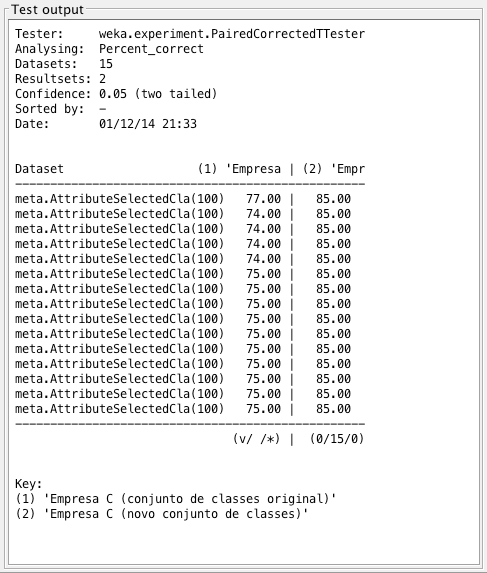
\includegraphics[width=\textwidth]{figs/empresa_c/exaustive-j48.png}
	\caption{\label{fig_17}Aplicação exaustiva do J48 para a Empresa C}
\end{figure}
\clearpage

\begin{figure}[p]
	\centering
	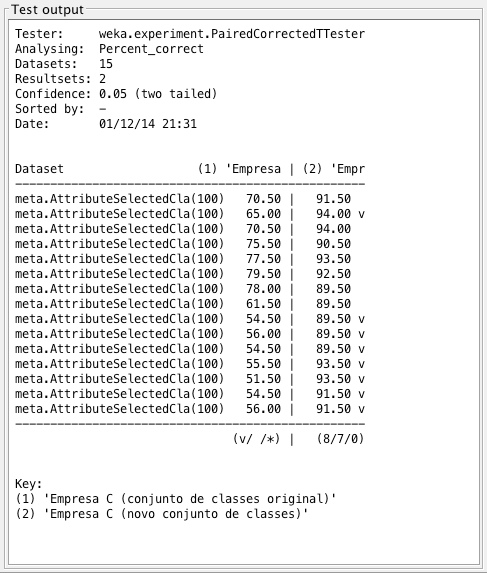
\includegraphics[width=\textwidth]{figs/empresa_c/exaustive-naivebayes.png}
	\caption{\label{fig_18}Aplicação exaustiva do NaïveBayes para a Empresa C}
\end{figure}
\clearpage